\section{Question 4 }\label{sec:q4}    
\subsection{4a}
\begin{figure}[H]
    \centering
    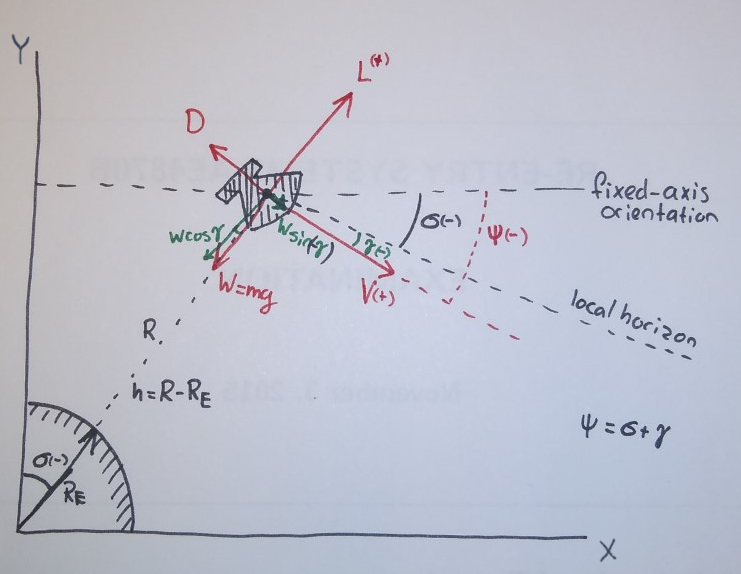
\includegraphics[width=0.9\columnwidth]{Figures/picture_EOM.jpg}
    \caption{Framework from which to derive equations of motion}
    \label{fig:eom}
\end{figure}

\subsection{4b}
We start with linear momentum parallel to velocity V. We can then find using Newton's second law that:
\begin{equation}\label{eq:eom1}
    m \frac{dV}{dt} = -D - m g sin(\gamma)
\end{equation}
This is the first of the equations of motion that we need to find. The second one we can find by looking at how the length of R changes:
\begin{equation} \label{eq:eom3}
    \frac{dh}{dt} = V sin(\gamma)
\end{equation}
Finally, we look at the normal acceleration, from which we obtain that:
\begin{equation}\label{eq:eom2}
    m V \frac{d\psi}{dt} = L - m g cos(\gamma)
\end{equation}
We would like to have things in terms of $\gamma$ rather than $\psi$, so first we need to transform this. First, we can see from the figure that there is a direct relation between these two angles.
\begin{equation}
    \psi = \sigma + \gamma
\end{equation}
and therefore:
\begin{equation} \label{eq:ihateangles}
    \frac{d\psi}{dt} = \frac{d\sigma}{dt} + \frac{d\gamma}{dt}
\end{equation}
Great, but now we also need an expression for $\frac{d\sigma}{dt}$. Due to the fact that position vector R is describing an instantaneous circular motion, we can relate the tangential velocity of this motion with the projection of V onto the local horizon, as they are equal:
\begin{equation}
    R\frac{d\sigma}{dt} = -V cos(\gamma)
\end{equation}
If we combine this with equation \ref{eq:ihateangles}, we find:
\begin{equation}
    \frac{d\psi}{dt} = -\frac{V}{R} cos(\gamma) + \frac{d\gamma}{dt}
\end{equation}
This we can now substitute into \ref{eq:eom2}:
\begin{equation}
\begin{split}
    m V \left( -\frac{V}{R} cos(\gamma) + \frac{d\gamma}{dt} \right) = L - m g cos(\gamma) \\
    m V \frac{d\gamma}{dt} = L - m g cos(\gamma) + m \frac{V^2}{R} cos(\gamma) \\
    m V \frac{d\gamma}{dt} = L - m g cos(\gamma) \cdot \left(1 - \frac{V^2}{gR} \right) \\
    m V \frac{d\gamma}{dt} = L - m g cos(\gamma) \cdot \left(1 - \frac{V^2}{V_c^2} \right)\\
\end{split}
\end{equation}
where $V_c = \sqrt{gR}$. This is our third equation of motion.

\subsection{4c}
Our starting point is the given expression for $V/V_E$:
\begin{equation}\label{eq:vratio}
    \frac{V}{V_E} = exp \left( \frac{g \rho}{2 K \beta sin(\gamma_E)} \right)
\end{equation}
and the first equation of motion:
\begin{equation}\label{eq:eom1b}
    m \frac{dV}{dt} = -D - m g sin(\gamma)
\end{equation}

First, we define the deceleration $\bar{a}$ as:
\begin{equation}
    \bar{a} = - \frac{dV}{dt}
\end{equation}
Furthermore, we assume that since re-entry motions generally occur at high velocities, the drag forces far exceed the weight components of the vehicle (i.e. $D \gg W$). This allows us to ignore the weight-related term of equation \ref{eq:eom1b}. Now we do some recreational algebra to find an expression for the deceleration.

\begin{equation} \label{eq:a1}
\begin{split}
    m \bar{a} = m -\frac{dV}{dt} = + D - m g sin(\gamma) = D\\
    \bar{a} = \frac{D}{m} = \frac{C_D \rho S V^2 }{2 m} \frac{g}{g} = \frac{\rho V^2 g}{2 K}\\
\end{split}
\end{equation}
Where we introduced the weight-referenced ballistic coefficient, defined as:
\begin{equation}
    K = \frac{m g}{C_D S}
\end{equation}
The relation we have found so far has a term for density, so it is helpful to unpack this variable to see how it influences the deceleration. But we can solve equation \ref{eq:vratio} for $\rho$ and put that in \ref{eq:a1}.

\begin{equation} \label{eq:densitystuff}
\begin{split}
    \frac{V}{V_E} = exp \left( \frac{g \rho}{2 K \beta sin(\gamma_E)} \right) \\
    ln \left( \frac{V}{V_E} \right) = \frac{g \rho}{2 K \beta sin(\gamma_E)} \\
    \rho = \frac{2 K \beta sin(\gamma_E) ln(\frac{V}{V_E})}{g} \\
\end{split}
\end{equation}

We now substitute this into \ref{eq:a1}:
\begin{equation}
    \bar{a} = \beta sin(\gamma_E) V^2 ln \left( \frac{V}{V_E} \right)
\end{equation}

We now apply a trick by multiplying and dividing this by a factor $V_E^2$. We do this because it will be easier to differentiate if we use $V/V_E$ as differentiation variable.

\begin{equation} \label{eq:a3}
    \bar{a} = \beta sin(\gamma_E) V_E^2 \left( \frac{V}{V_E} \right)^2 ln \left( \frac{V}{V_E} \right)
\end{equation}

Ultimately, we want to know when the deceleration is maximal. The approach is to differentiate equation \ref{eq:a3} and figure out when this is zero. As mentioned, we differentiate with respect to $V/V_E$:

\begin{equation} \label{eq:dadv}
\begin{split}
    \frac{d\bar{a}}{d(V/V_E)} = 2 \beta sin(\gamma_E) V_E^2 \frac{V}{V_E} ln \left( \frac{V}{V_E} \right) + \beta sin(\gamma_E) V_E^2 \left( \frac{V}{V_E} \right)^2 \left( \frac{1}{V/V_E} \right) \\
    = \beta sin(\gamma_E) V_E^2 \left[ 2 + ln \left( \frac{V}{V_E} \right) \right] \frac{V}{V_E} = 0 \\
\end{split}
\end{equation}
This is only equal to zero if:
\begin{equation}
\begin{split}
    2 ln \left( \frac{V'}{V_E} \right) = -1 \\
    \frac{V'}{V_E} = e^{-1/2} = \frac{1}{\sqrt{e}}
\end{split}
\end{equation}
This means that the maximum deceleration occurs when the velocity of the vehicle is about $61\%$ of the entry velocity. We can substitute this result into \ref{eq:a3} to find the corresponding deceleration.
\begin{equation} \label{eq:a4}
    \bar{a}_{max} = \beta sin(\gamma_E) V_E^2 \cdot (e^{-1/2})^2 \cdot ln (e^{-1/2}) = -\frac{\beta sin(\gamma_E)}{2 e} V_E^2
\end{equation}

\subsection{4d}
Just a matter of plugging the right values into equation \ref{eq:a4}. Use $\beta = 1/H_s$ to find $\beta$.
\begin{equation}
    (\bar{a}_{max})_{\venus} = - \frac{15900^{-1} \cdot sin(-32.4 ^\circ)}{2 e} \cdot 11670^2 = 844.2 \, m/s^2
\end{equation}
Similarly, we can find the other decelerations:
\begin{equation}
\begin{split}
    (\bar{a}_{max})_{\oplus} = 1903.9 \, m/s^2 \\
    (\bar{a}_{max})_{\mars} =  1525.3 \, m/s^2 \\
\end{split}
\end{equation}

\subsection{4e}
For this question, we use equation \ref{eq:densitystuff} and fill in the velocity ratio for maximal deceleration. This density $\rho'$ is the density of the air when maximum deceleration occurs. Then we can extract the corresponding altitude $h'$ from this density.
So we start with:
\begin{equation}
    \rho' = \frac{2 K \beta sin(\gamma_E) ln(\frac{V}{V_E})_{\bar{a}_{max}}}{g} = \frac{2 K \beta sin(\gamma_E) ln(\frac{1}{\sqrt{e}})}{g} = -\frac{K \beta sin(\gamma_E)}{g}
\end{equation}
Since we also assume that density varies exponentially with altitude, we have:
\begin{equation}
\begin{split}
    \rho' = -\frac{K \beta sin(\gamma_E)}{g} = \rho_0 e^{- \beta h'} \\
    -\beta h' = ln \left( -\frac{K \beta sin(\gamma_E)}{g \rho_0} \right) \\
    h' = \frac{1}{\beta} ln \left( -\frac{g \rho_0}{K \beta sin(\gamma_E)} \right) \\
\end{split}
\end{equation}

\subsection{4f}

This result from the previous question can be used to find the three altitudes we need. However, the weight-referenced ballistic coefficient K for the lander on each planet is still unknown, so we have to find those first:

\begin{equation}
    K_{\venus} = \frac{mg}{c_D S} = \frac{8.87 \cdot 315}{1.1 \cdot \pi/4 \cdot 1.4228^2} = 1598 \, \left[ \frac{kg}{m \cdot s^2} \right]
\end{equation}
And for the other planets:
\begin{equation}
\begin{split}
    K_{\oplus} = 1767\, \left[ \frac{kg}{m \cdot s^2} \right] \\
    K_{\mars} =  671.3 \, \left[ \frac{kg}{m \cdot s^2} \right] \\
\end{split}
\end{equation}

Now for the corresponding altitudes:
\begin{equation}
\begin{split}
    h'_{\venus} = 15900 ln \left( -\frac{8.87 \cdot 65}{15900^{-1} 1598 sin(-32.4^{\circ})} \right) = 147.5 \, km\\
    h'_{\oplus} = 31.68 \, km\\
    h'_{\mars} = 3.75 \, km\\
\end{split}
\end{equation}

\subsection{4g}
To answer this question, we want an equation that relates parachute diameter (since a circular planform is used) to a landing velocity $V_f$. We can find this relation by first looking at the forces acting on the vehicle and parachute.

\begin{figure}[H]
    \centering
    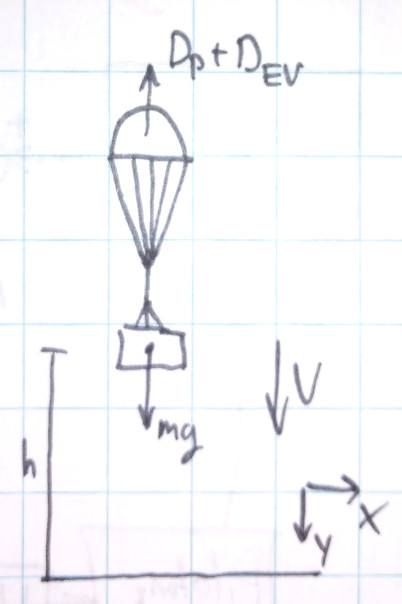
\includegraphics[width=0.3\columnwidth]{Figures/chute_fbd.jpg}
    \caption{Simple FBD of the vehicle and parachute.}
    \label{fig:chute_fbd}
\end{figure}
Since we can neglect the drag of the vehicle, $D_{EV} = 0$ and all the drag is generated by the parachute, i.e. $D = D_p$.
Applying Newton's second law to the diagram in the positive Y-direction, we get:
\begin{equation}
    m \frac{dV}{dt} = -D_p + mg = -\frac{1}{2} C_{D_p} \rho S_p V^2 + mg 
\end{equation}
When the parachute is near the ground, we should be in a situation where the vehicle is no longer decelerating but drifting down at constant speed. So we assume that we have $\frac{dV}{dt} = 0$, and then solve the previous equation for $S_p$:
\begin{equation}
\begin{split}
    \frac{1}{2} C_{D_p} \rho S_p V_f^2 = mg\\
    S_p = \frac{2 m g_0}{C_{D_p} \rho V_f^2}\\
\end{split}
\end{equation}
Note that we have changed $V$ to the final velocity $V_f$, as the speed no longer changes. For a circular parachute planform, can find the parachute diameter:
\begin{equation}
    d_p = \sqrt{\frac{8}{\pi} \frac{ m g_0}{C_{D_p} \rho V_f^2}}
\end{equation}
And so on Earth you would need:
\begin{equation}
    (d_p)_\oplus = \sqrt{\frac{8}{\pi} \frac{315 \cdot 9.81}{0.512 \cdot 1.225 \cdot 10^2}} = 11.2 \, m
\end{equation}

\subsection{4h}
Using the exact same relation as in the previous question:
\begin{equation}
\begin{split}
(d_p)_{\venus} = 1.46 \, m \\
(d_p)_{\mars} = 59.0 \, m \\
\end{split}
\end{equation}

\subsection{4i}
In terms of deceleration, the Earth seems the most demanding case, owing to the high value of $\bar{a}_{max}$ compared to Mars and Venus. This means for an Earth re-entry, the structure will have to be the strongest, and this may increase the structural mass of the re-entry vehicle. It also has other consequences if there are people on board, who will have to survive these decelerations, and so if the peak deceleration is too high, a redesign may have to be in order. Venus is the most favourable planet in terms of maximum deceleration (so if astronauts ever want to travel to its surface, at least it won't be the re-entry deceleration peak that kills them). \\
Owing to its dense atmosphere, a Venus lander also requires a vastly smaller parachute size, which can reduce vehicle mass because the parachute will be lighter, and potentially less complex. In comparison, the same lander on Mars would require about forty times the parachute diameter compared to the one needed for a Venus landing. For Earth, this factor is about ten times, and so it fits somewhere in between.